\documentclass[border=0pt]{standalone}
\usepackage[utf8]{inputenc}
\usepackage{graphicx}
\usepackage{subcaption}
\usepackage{tikz}
\usepackage{float}
\usepackage[dvipsnames]{xcolor}
\usetikzlibrary{matrix, positioning,calc,arrows.meta, backgrounds,fit,shapes.geometric}
\tikzset{
    every node/.style={font=\small},
    greencycle/.style={fill=green!80!black!10,ellipse, align=center},
    rectred/.style={draw=red, fill=green!80!black!10, thick, rounded corners, align=center},
    rectblue/.style={draw=blue, rounded corners, align=center},
    yellowbox/.style={draw=black, fill=Dandelion, thick, rounded corners, align=center},
    bluecycle/.style={fill=NavyBlue, ellipse, align=center},
    arrow/.style={-{Latex[length=3mm]}, thick},
}

\begin{document}
\begin{minipage}{6.75in}
\centering
\captionsetup{type=figure}
\begin{subfigure}[b]{0.45\linewidth}\centering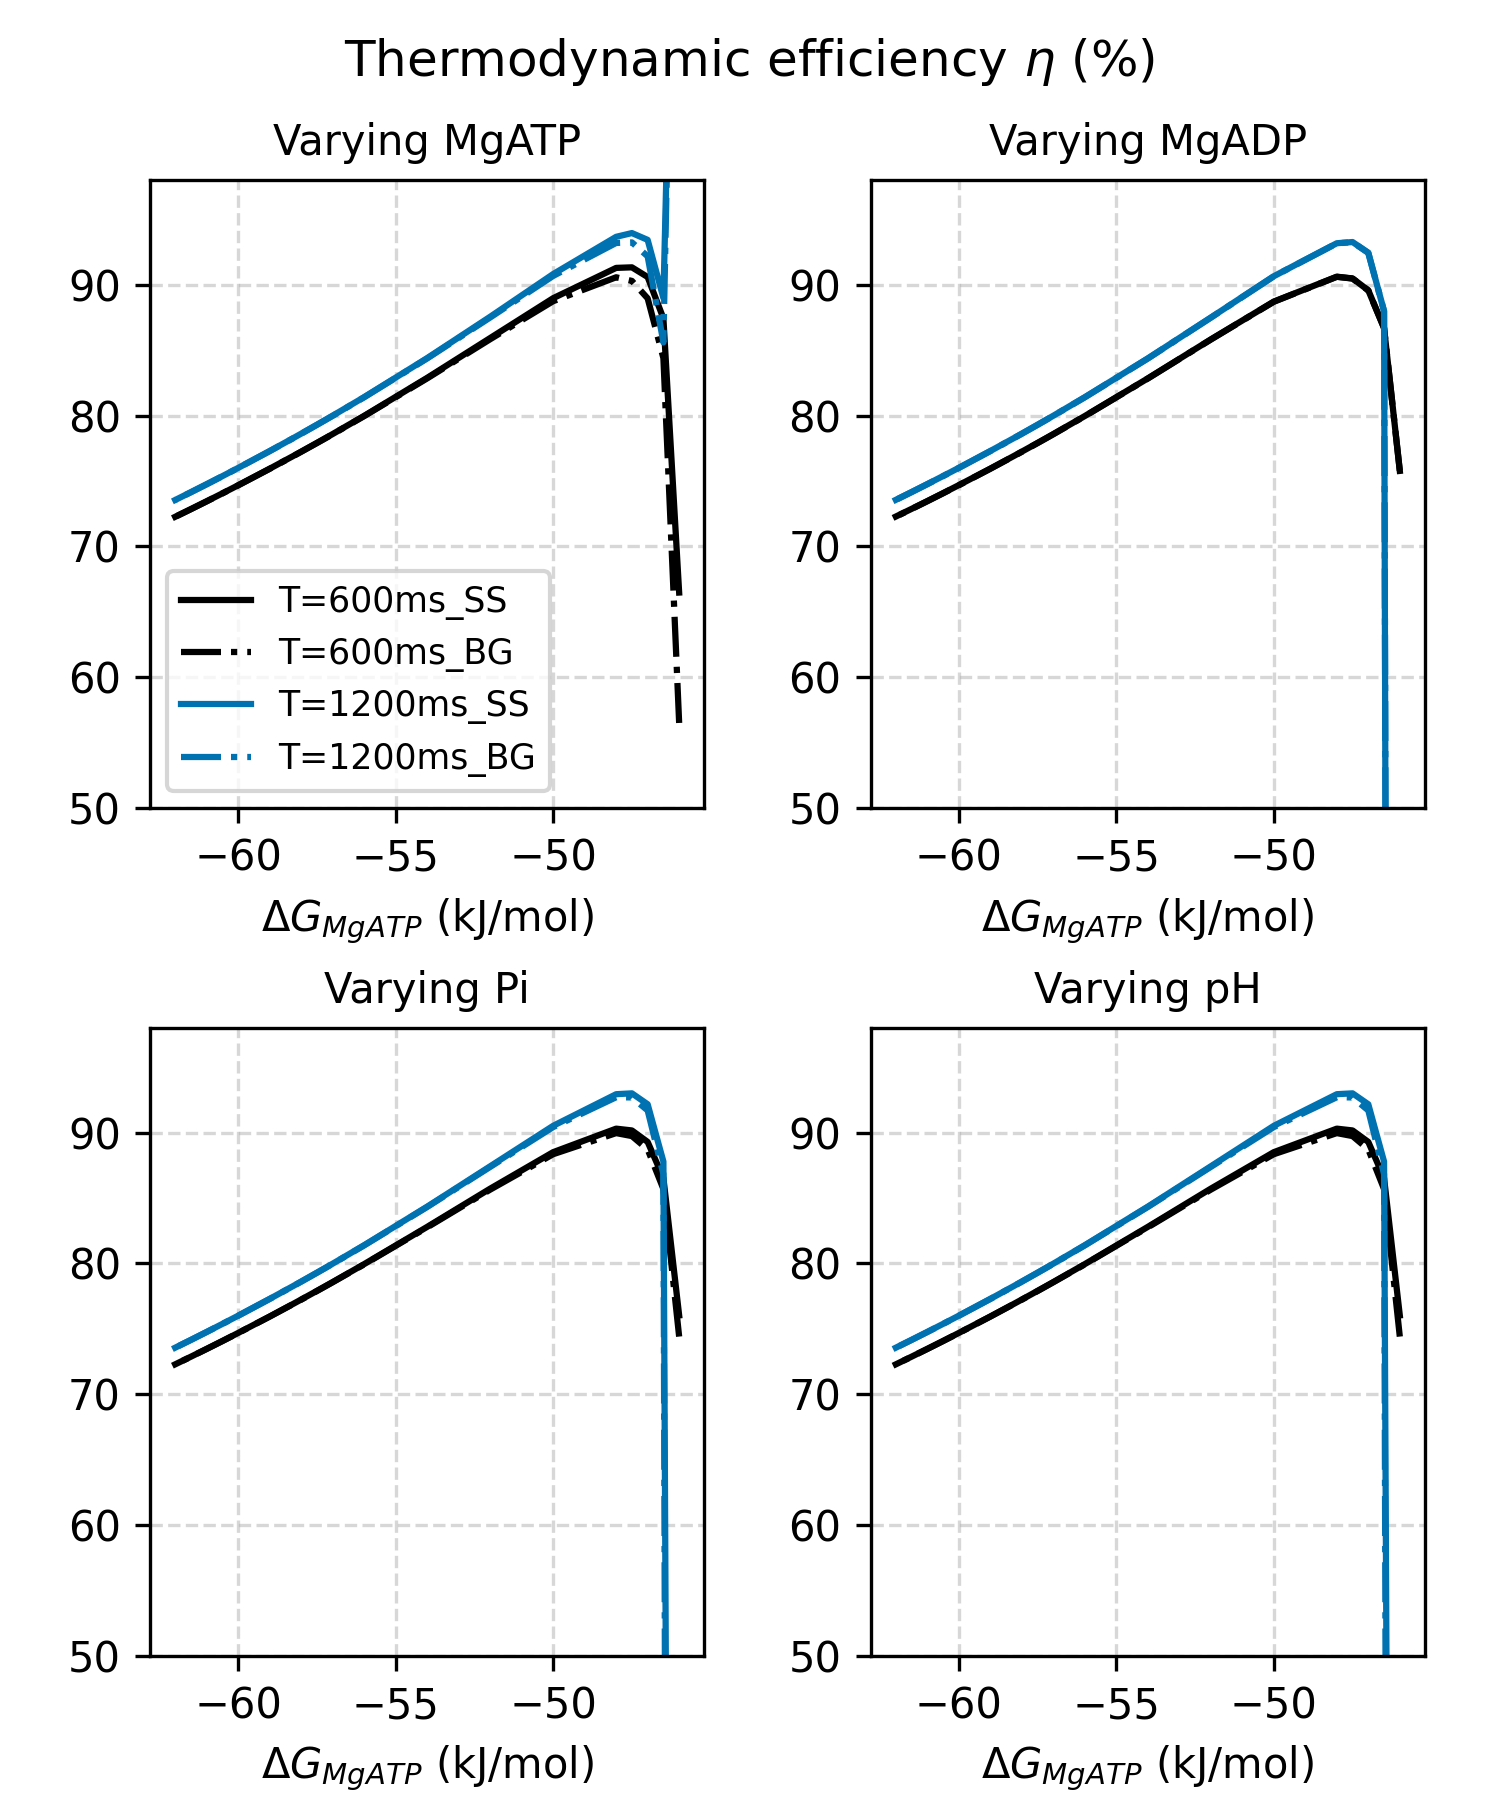
\includegraphics[width=\linewidth]{6stateV2_Thermodynamic_efficiency_deltaATP_2.png}\caption{6-state model}\end{subfigure}
\begin{subfigure}[b]{0.45\linewidth}\centering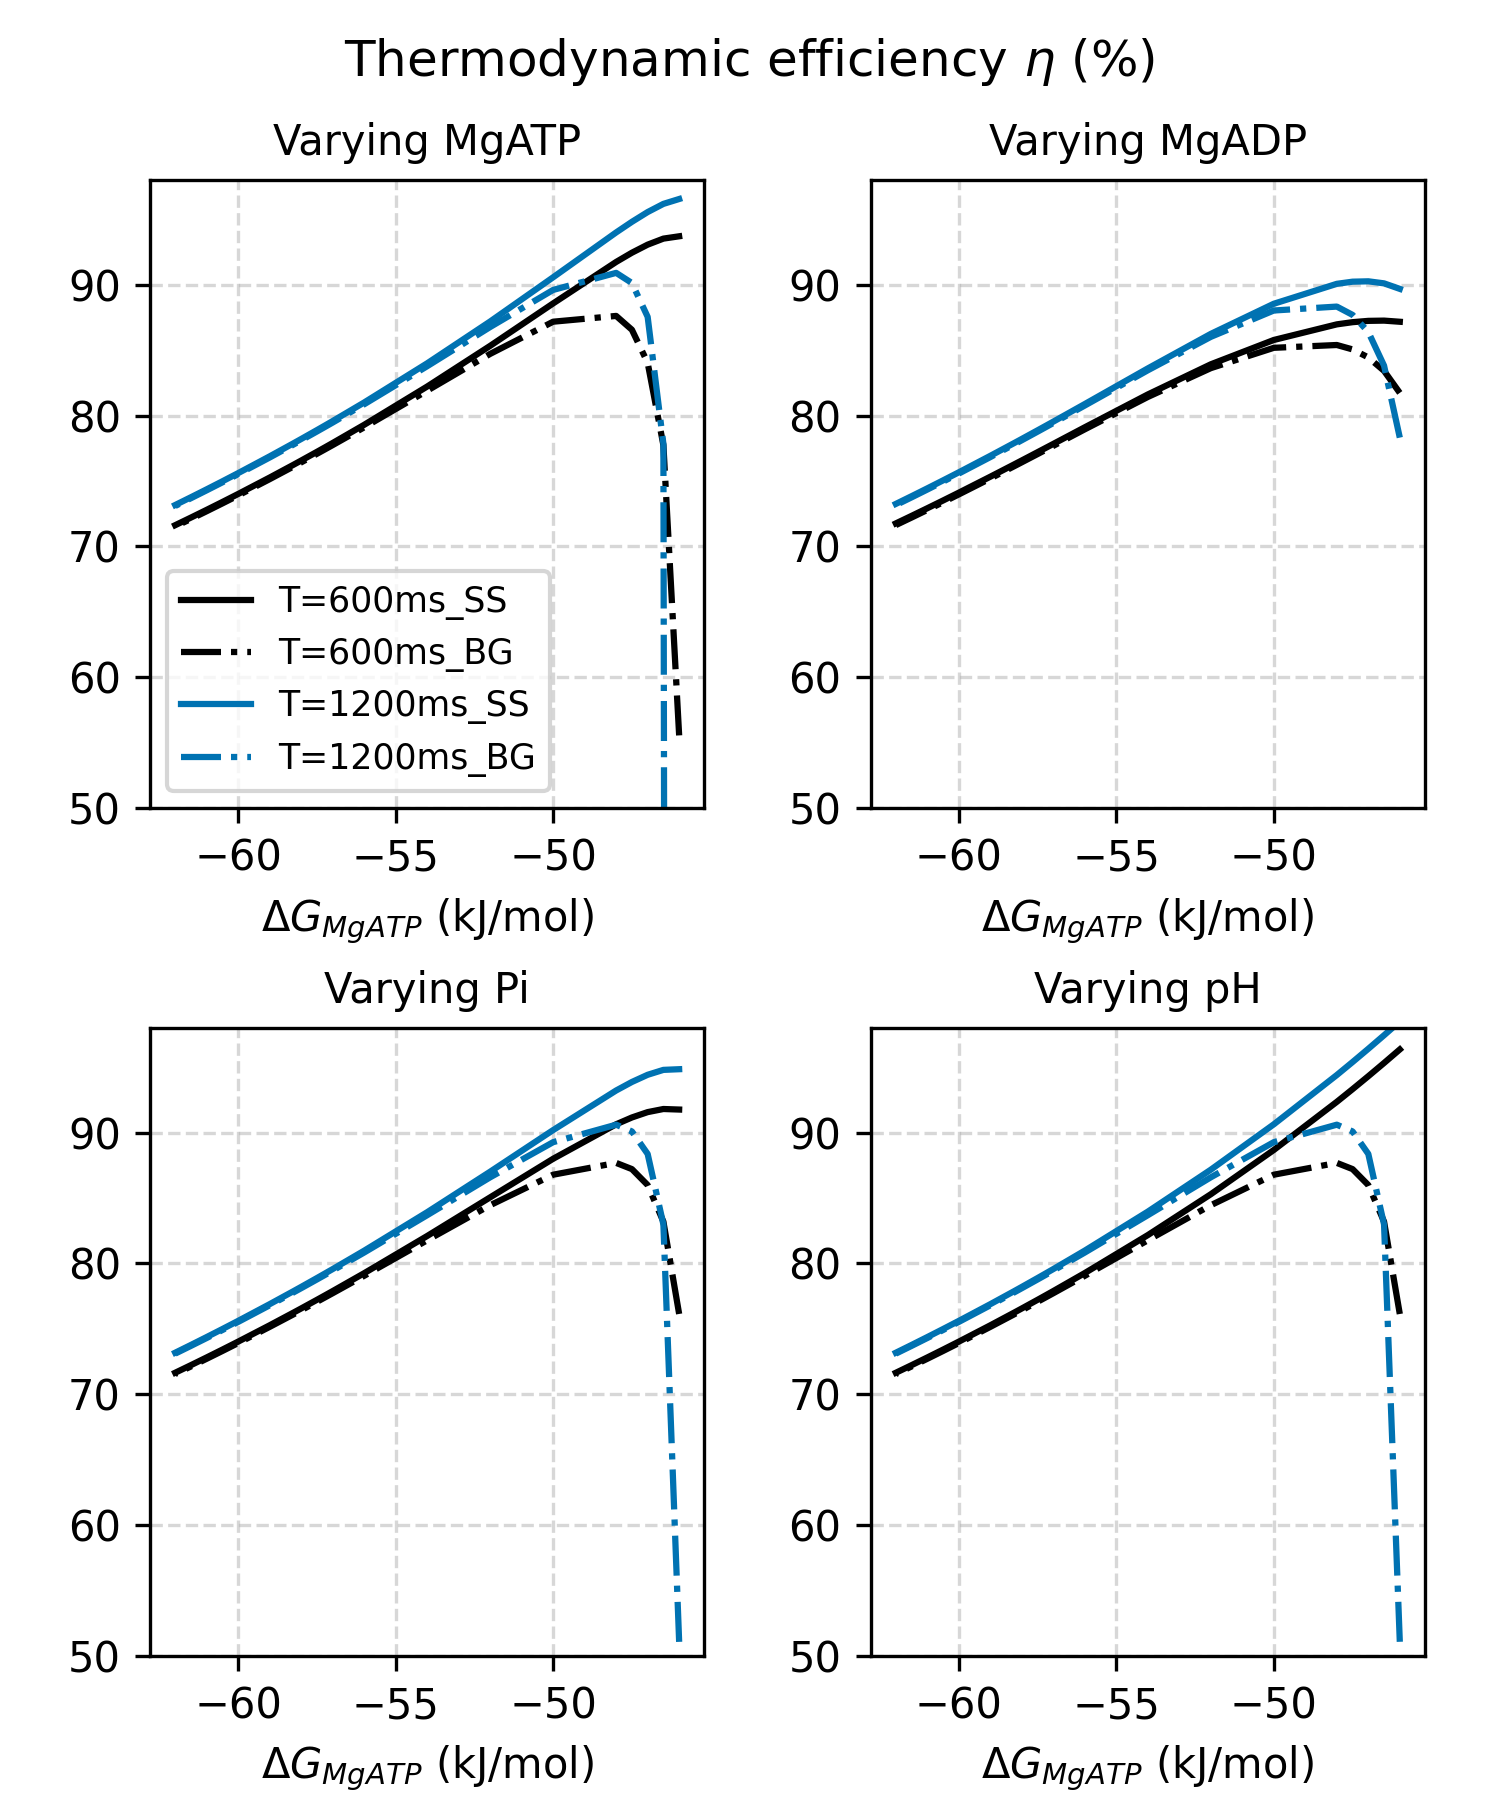
\includegraphics[width=\linewidth]{15state_Thermodynamic_efficiency_deltaATP_2.png}\caption{15-state model}\end{subfigure}
\end{minipage}
\end{document}
